\chapter{\IfLanguageName{dutch}{Stand van zaken}{State of the art}}%
\label{ch:stand-van-zaken}

\section{\IfLanguageName{dutch}{GraphQL}{GraphQL}}%
\label{sec:GraphQL}

In deze sectie van de literatuurstudie spitsen we ons toe op de eerste deelvraag van dit onderzoek: “Wat is GraphQL?”
De hier opvolgende secties zijn opgesteld naarmate de benodigde onderdelen die helpen een beter beeld te scheppen over de werking van GraphQL en hoe deze software tot stand is gekomen.

Hierbij zal er ook meer uitleg gegeven worden over de samenstelling van GraphQL en wat deze onderdelen exact inhouden. Dit zal dan duiding geven voor welke doeleinden men deze software gebruikt. Er wordt ook besproken welke gebruiksvoordelen er zijn ten opzichte van eerder traditionele software en hoe men in gebruik brengt.

Tot slot zullen API's uitgeklaard worden en een startpunt geven om de Data Accelerator voor te stellen.

\subsection{\IfLanguageName{dutch}{Gegevens ophalen}{Fetching data}}%
\label{sec:Gegevens ophalen}
In 2012 creëerde Facebook GraphQL omdat men binnen het bedrijf op zoek was naar een betere manier om data op te halen, om zo hun mobiele applicaties herop te bouwen. Voorheen werd er bij hun iOS en Android apps gebruik gemaakt van een omvorming van hun website. Dit zorgde op termijn dat naarmate de applicaties uitgebreider werden, er zich meer problemen rondom geleverde prestaties en functioneren voordeden.

 De oplossing hiervoor moest toepasbaar zijn over de hele lijn van producten en diensten waarover het bedrijf beschikte. De software zelf moest op zijn beurt verstaanbaar zijn voor zowel de ontwikkelaars, ontwerpers evenals collega’s die niet over technisch voorkennis beschikten. Na enkele jaren intern te hanteren is deze software publiek gesteld in 2015. Facebook hun doel van de software was een makkelijkere manier ontwikkelen om benodigde data op te halen zonder dat hun applicatie ontwikkelaars weten welke bronnen er exact gehanteerd werden.\autocite{GraphQLFoundation2022}

\subsection{\IfLanguageName{dutch}{Querytaal}{Query language}}%
\label{sec:Querytaal}
De naam GraphQL is een samenstelling van twee woorden, Graph en QL. Het deel QL staat voor Query Language en zal benoemd worden doorheen deze bachelorsproef als querytaal. Een querytaal is een manier van schrijven met als doel data of informatie uit één of meerdere tabellen van een databank te verkrijgen. In de meeste instanties bestaat een databank uit verschillende rijen en tabellen bevattende data omtrent een speciefiek thema zoals gegevens van werknemers. De data verkrijgen verloopt aan de hand van een verzoek, de query, die specificeert welke data uit de gebruikte databank benodigd is. Die query bestaat uit een vastgelegde werkwijze van coderen zodat de databank het verzoek begrijpt en kan verwerken.Via een query kan je de tabel met gegevens aanspreken om de gewenste data op te vragen, aan te passen, sorteren en uiteindelijk weergeven aan de gebruiker naar gelang de gebruikte commandos in het verzoek.

Een query binnen GraphQL is een string die verstuurd wordt naar een server. Na het ontvangen van de query zal de server deze interpreteren en het verzoek vervullen. Als de gewenste data of operatie uitgevoerd is, zal de server een JSON sturen naar de client. De queries zijn gevormd naar de structuur van het verwachte antwoord. Op die manier kan men de query opstellen naar gelang de benodigde data voor een applicatie. Een query binnen GraphQL is ook onderverdeeld in niveaus, waarbij elk niveau overeenstemt met een type dat een set van velden bevat. Deze types kunnen via een query uit een GraphQL server opgevraagd worden. Door dat de query personaliseerdbaar is qua vorm naar de opstelling van de client, kan men de servers simplistischer en meer gegeneraliseerd maken.\autocite{Byron2015}

\subsection{\IfLanguageName{dutch}{Graaf}{Graph}}%
\label{sec:graaf}
Het andere deel van GraphQL's naam is Graph of graaf. Een graaf wordt gedefinieerd als een object bestaande uit een verzameling van een groep punten benoemd als knopen en hun onderlinge verbindingen, genaamd bogen. Elke boog zorgt voor de verbinding van twee knopen. Een verbinding kan ook een pijl bevatten om zijn richting aan te tonen. Op deze manier kunnen de relaties tussen verscheidene knopen in beeld gebracht worden. De boog op zich kan ook nog extra informatie bevatten, in dat geval hebben we een gewogen graaf. Binnen omgevingen waar men data ordent volgens een hiërarchische structuur zoals bestandssystemen, maakt men gebruik van bomen en grafen om de data te modelleren.\autocite{Lievens2021} In het werkstuk van \textcite{Brysbaert2021} wordt dit voorgesteld als een schema waarbij de knopen gebruikers zijn van het sociale media platform facebook en bogen de onderlinge vriendschap voorstellen. De bogen bevatten ook een pijl naar beide richtingen, omdat een vriendschap op het platform een wederzijdse toepassing is. In dit geval is de graaf dus ongericht. Dit is niet altijd een vereiste.

De hierboven uitgelegde werking kan men ook toepassen op een bestaande databank. Er zijn verbindingen tussen verschillende soorten data die elk ook hun specieke kenmerken bevatten. Via GraphQL kan men dus hierop inspelen en dichter op de actuele werking van een databank te werk gaan.

Juist omdat grafen zo dicht aansluiten bij de realiteit als men een model opstelt in gedachte houdende de processen die men moet doorlopen, kan men dit implementeren in een werkomgeving. Gebruikmakende van GraphQL, kan men een model opstellen volgens een graaf steunend op een schema. Binnen dit schema worden de knopen en hun onderlinge relaties vastgelegd. Aan de client zijde kan dit dan een vergelijkende weergave vormen zoals bij object georiënteerd programmeren. Enerzijds types die onderlinge referenties bevatten en anderzijds kan men voor de backend zowel hun oude of nieuwe instanties gebruiken.\autocite{GraphQLFoundation2022}

\subsection{\IfLanguageName{dutch}{Gebruik}{Usage}}%
\label{sec:Gebruik}
Bij de sterke punten van GraphQL hoort toch wel de preventie van over- en underfetching. Overfetching is een probleem die zich vaak voordoet bij eerder traditionele programmas zoals REST, waarbij er te veel data opgevraagd wordt ten opzichte van wat benodigd is. Gebruikmakend van GraphQL kan men zich toespitsen op juist de data die van toepassing is. Dit zorgt voor een lager verbuik van bandbreedte, dat voordelig is als men ook gebruikt maakt van mobiele aparaten zoals ook Facebook doet.\autocite{Byron2015} Het omgekeerde kan zich echter ook voor doen, bij underfetching wordt niet alle opgevraagde data weergeven in één keer. Dit kan voorgesteld worden als een boodschappenlijstje bij een grootwarenhuis of online winkel waarbij er voor elke productbeschrijving een individuele query zou moeten uitgevoerd worden. Dit is ook een probleem waar GraphQL op inspeelt door gebruik te maken van een hiërarchische opstelling. De onderlinge relaties tussen objecten wordt zo natuurlijk mogelijk behouden.

Voor ontwikkelaars is het ook handig dat GraphQL declaratief is, op deze manier is de data makkelijker te hanteren en zijn de queries overzichtelijker. Men kan ook gebruik maken van nesting om gerelateerde data op te vragen en om de queries zelf consistent te houden gedurende het hele proces. Via deze werkwijze moeten er dan ook geen responses samengevoegd worden. GraphQL bezit ook schemas die kunnen dienen als een contract om front-end apps te ontwikkelen (dit gebeurt door de API verzoeken te simuleren). Het back-end team kan het contract dan later aanleveren met de nodige diensten. Binnen een graaf moeten de ontwerpers maar over een enkele endpoint beschikken om toegang te hebben tot de achterliggende data.

\subsection{\IfLanguageName{dutch}{API}{API}}%
\label{sec:API}
Een Application Programming Interface, beter gekend als API, staat in voor de communicatie tussen een client en een server. Vanuit de client wordt er een verzoek gestuurd naar de corresponderende server met de benodigde gegevens voor het verzonden request. De server op zijn beurt zal dan het verzoek verwerken en een gepaste respons sturen naar de client. Hierna zal de respons omgevormd worden en beschikbaar gesteld worden aan de gebruiker op een duidelijke wijze. Via de vernoemde client kan men gebruik maken van een request om gegevens naar een databank te sturen of om data juist op te vragen. Dit gebeurt aan de hand van een API. Deze is als het ware de tussenpersoon tussen de client en de server.\autocite{Willem2021}

Een API stelt duidelijke regels vast omtrent de communicatie en steunt hierbij op het client-servermodel. Dit model zorgt ervoor dat computersystemen onderling kunnen samenwerken. De client zal bij de start van de communicatie altijd als eerste de server contacteren. Hierbij staat de server in voor de clients omtrent het aanbieden van diensten, in de vorm van programma's. In het geval van deze bachelorproef zal er voornamelijk naar data gekeken worden, maar de diensten kunnen ook de vorm aannemen van berekeningen of andere operaties.

De diensten die met data omspringen waar zich op toegespits zal worden, zullen vooral in lijn liggen met het converteren, uitvoeren, queryen en transformeren. Dit staat ook gekend als delen van CRUD. Dit acroniem staat voor Create, Read, Update en Delete.\autocite{Martin1983} Het acroniem is een samenvatting voor alle operaties die men kan uitvoeren om data te manipuleren. Hierbij maakt men gebruik van een API. Er wordt gebruik gemaakt van een relationele databank om de persistentie van de data te regelen.

Een API is handig om te gebruiken vanwege de veelzijdigheid van opties. Men kan software die instaat voor de implementatie verbergen zodat het voor concurrenten moeilijker is om te weten te komen hoe het programma exact in werking treed. Op die manier wordt het intellectuele eigendom beschermd en behoudt men zijn voordelen ten opzichte van concurrentie. Door het verborgen houden van code kunnen mensen die misbruik willen maken hiervan om zo toegang tot het programma te verkijgen of de werking stop te zetten, een extra hindernis opgelegd worden. Zoals vernoemd in de sectie van grafen, kan men ook nieuwe instanties creëren of aanpassingen doorvoeren zonder dat de clients of andere systemen die de API gebruiken, niet aangepast dienen te worden.\autocite{Martin2017}

\section{\IfLanguageName{dutch}{Data-Accelerator}{Data-Accelerator}}%
\label{sec:Data-Accelerator}

Deze sectie zal zich toespitsen op de tweede deelvraag van het onderzoek: “Wat is een Data-Accelerator?”. Herbij zal er in de volgende secties emer uitleg gegeven worden in verband met de geschedenis van de software en diens verschillende toepassingen. Op deze manier kan er duiding gegeven worden omtrent het bestaan van de Data-Accelerator en waarom men bij Delaware hier verder wil op inzetten. Tot slot zal er ook uitgelegd worden wat er benodigd is om deze te kunnen gebruiken.

\subsection{\IfLanguageName{dutch}{Microsoft Azure}{Microsoft Azure}}%
\label{sec:Microsoft Azure}

Microsoft Azure is de benaming die gegeven is aan de cloud computing services van Microsoft. Dit bevat een complex en breed aanbod van services die nog steeds ondersteuning krijgen en verder uitgebreid worden. Azure is nu ondertussen toch al veertien jaar geleden geïntroduceerd in 2008 en is sindsdien substantieel gegroeid in hun capaciteiten en divers aanbod. Voor 2008 werd er binnen Microsoft zich vooral gefocust op een andere cloud service die gekend was onder de naam Business Productivity Online Standard Suite of BPOS kort gezegd. Deze bestond uit software pakketten zoals Exchange2007, Office Communications Online, Microsoft Office Sharepoint Server2007, Microsoft Office Live Meeting en Office Communications Online.

Echter in 2011 heeft Microsoft de naamgeving aangepast van BPOS naar Office365. Dit kwam in de vorm van Software as a Service of SaaS. Dit concept hield in dat klanten niet langer meer infrastructuur moesten voorzien voor hun tools, maar deze via een subscriptie toegang konden krijgen. Aan dit softwarepakket werd dan ook Exchange Online toegevoegd om dus ook e-mail services te voorzien. Nog een toevoeging was SharePoint Online. Later kwam hier ook Lync Online voor directe berichtgevingen en virtuele vergaderruimtes op te zetten. Het laatste deel van dit pakket was Office Pro Plus om ook de functionaliteiten te voorzien voor zowel computer als mobiele gebruikers.

Om deze SaaS producten te voorzien voor klanten, heeft Microsoft enkele datacenters moeten bouwen, zowel voor BPOS als later Office365. Deze datacenters worden bij Microsoft zelf onderhouden door het Global Foundation Services team. Het gevolg hiervan is dat de klanten van deze Microsoft services de optie hebben om gebruik te maken van deze functionaliteiten zonder extra complexiteit die met het onderhouden hiervan gepaard gaat. De voordelen van deze services zijn ook dat deze gemakkelijk schaalbaar, beschikbaar en bijhorende service-level agreements. Hiervoor waren er meer datacenters, opties om wereldwijd te werk te gaan en goed opgeleide werknemers nodig. Door deze toepassingen waren niet alleen voor grote, maar ook voor kleine bedrijven deze service-level agreements een mogelijke optie.

Om zeker te zijn dat deze services de bepaalde prestaties halen, werden er monitoring tools zoals System Center Operations Manager voorzien. Ook om Office365 gebruikers ongelimiteerd OneDrive opslag ruimte te geven, moest er bij de GFS een oplossing bedacht worden. Dit moest dan op zijn beurt wel competitief zijn met andere marktspelers, dus het economische aspect bij operaties op die schaal en de efficiëntie hierbij waren belangrijke aspecten voor Microsoft en het GFS team.

Cloud computing is dan ook ontstaan door het capitaliseren op de mogelijkheid om computerberekeningen extern te realiseren. Azure veronderscheidde zich hierin door volledig toe te spitsen op het voorzien van deze cloud services. Hiervoor was Azure dus ook volledig van nul opgebouwd om Office36 te kunnen ondersteunen en open te stellen voor andere sevices zoals Active Directory.\autocite{Copeland2015}

\subsection{\IfLanguageName{dutch}{IaaS, PaaS en SaaS}{IaaS, PaaS en SaaS}}%
\label{sec:IaaS, PaaS en SaaS}

Microsoft Office365 kan dus gezien worden als Software as a Service of SaaS. Er zijn ook nog andere types van cloud services zoals Infrastructure as a Service of IaaS en Platform as a Service of PaaS. Infrastructure as a Service wordt gezien als de combinatie van het draaien of hosten, voorzien van hardware en basis services om een cloud te kunnen ondersteunen.
Het gebruik hiervan komt neer op het voorzien van toegang tot gedeelde middelen op basis van benodigdheden, zonder dat er details in verband met locatie en de infrastructuur van clienten blootgesteld worden. Ook moeten details omtrent server images, een kopie van de server, opgevraagd kunnen worden, moet er opslag voorzien zijn en wachtrijen beschikbaar zijn. Hierbovenop moet de info van andere middelen die gebruikt worden ook opvraagbaar zijn.
De controle over de volledige infrastructuur van server en niet alleen van de applicaties, instanties en gebruikte containers is ook een gegeven. Nadelen hiervan zijn het management van de gebruikte middelen, de netwerk infrastructuur, de virtualisatie, data beheer en de gebruikte API's.\autocite{Manvi2014}

Zowel software evenals hardware als service hebben hun toegevoegde waarde in het bedrijfsleven bewezen. Platform as a Service of PaaS heeft als rol om het benodigde platform voor de virtuele middelen in de vorm van software te voorzien. Dit komt voor als een volledig afgewerkt platform bestaande uit hardware en software. Vanuit een economisch standpunt kan het PaaS model kan deze inspelen op verschilelde delen binnen de software wereld. Als eerste heb je de klanten, die via het voorziene netwerk hun Saas omgeving beschikbaar hebben. Ten tweede heb je de software ontwikkelaars die via het platform beter kunnen inspelen en ondersteuning bieden aan hun operatoren en ten derde heb je de bedrijven die vroeger de verantwoordelijkheid droegen om te zorgen dat de software correct geïmplementeerd werd samen met het voorzien van de benodigde infrastructuur.\autocite{Beimborn2011}

Omdat Azure berekeningskracht voor Office365 draagt, zoals Active Directory, is het evident om IaaS te antwoorden als we ons afvragen onder welke term Azure zich bevindt. Azure staat dan ook het meest bekend om hun IaaS aanbod zoals Azure virtual machines en virtuele netwerken. Ook horen hier de Azure storage solutions en recovery services bij. Er mag echter niet vergeten worden dat Azure ook een groot aanbod aan PaaS heeft. Enkele gekende voorbeelden hiervan zijn Azure SQL Database, Azure websites en het Azure Content Delivery Network. Hier bovenop komen ook nog eens de Azure BizTalk Services en de Azure Mobile Services. Hierdoor kan Microsoft als een van de weinige marktspelers een stevig aanbod van mature technologiën, infrasturctuur en financiële pakketten aanbieden omtrent IaaS, Paas en Saas.\autocite{Copeland2015}

\subsection{\IfLanguageName{dutch}{Ontstaan Data-Accelerator}{Ontstaan Data-Accelerator}}%
\label{sec:Ontstaan Data-Accelerator}

De Data-Accelerator is twee jaar geleden ontworpen binnen Delaware door Dhr. Simon Dedeken als een initieel idee om XSLT mappings uit te voeren. Voorheen werd dit gedaan bij klanten die gebruik maakten van Delaware hun services omtrent integratie binnen hun Azure omgeving in de vorm van een Integration Account. Vele klanten waren echter niet happig naar het extra kostenplaatje dat hieraan verbonden was. XSLT of eXtensible Stylesheet Language Transformation, is een taal om XML of eXtensible Markup Language, een standaard om documenten vast te leggen volgens een structuur, te transformeren in andere XML documenten. XSLT was ontworpen om gebruikt te worden bij XSL, die op zijn beurt de XML woordenschat bevat om het formaat te specifiëren. XSL wordt gebruikt om de vormgeving te specifiëren bij een XML document door gebruik te maken van XSLT om de benodigde transformatie te beschrijven ten opzichte van het gewenste XML document. XSLT kan ook zelfstandig werken zonder de benodigdheid van XSL, maar is niet ontworpen als een algemene XML transformatie taal. Het doel is voornamelijk om de transformaties te voorzien die benodigd zijn wanneer XSLT gebruikt wordt als een deel binnen XSL.\autocite{W3C1999}

Die mappings konden via het zelfgeschreven programma in C-sharp van Dhr. Dedeken uitgevoerd worden zowel lokaal als via een Function App in Azure. Later is hier dan ook ETL functionaliteit aan toegevoegd. Dit staat voor Extraction, Transformation en Load operaties met data in een databank. Van hier uit kwam het idee om de Data-Accelerator als een soort Zwitsers zakmes te gebruiken en verder uit te werken. Door de limitaties van Logic Apps in Azure kon er via deze Function App wel een generieke oplossing voorzien worden. Samen met een andere collega heeft Dhr. Dedeken hier dan ook conversies aan toegevoegd zoals JSON naar Excel en omgekeerd. Hedendaags wordt de Data-Accelerator gebruikt als een accelerator voor collegas in de vorm van een starter paket om generiek te werk te gaan. De naam accelerator werd hierbij gekozen omdat deze ook helpt om sneller te werk te gaan en extra functionaliteiten toe te voegen aan een project bij klanten van Delaware.\autocite{LopezNovoa2015}

\subsection{\IfLanguageName{dutch}{Werkomgeving}{Werkomgeving}}%
\label{sec:Werkomgeving}

In een werkomgeving wordt de Data-Accelerator gebruikt blij klanten die heel wat data versturen en ontvangen. Onder de naam klanten bevinden zich echter niet alleen bedrijven, maar ook functies en applicaties binnen het voorziene platform van een klant. Delaware heeft hiervoor een framework opgesteld binnen Azure aande hand van verworven kennis die verschillen Azure componenten die hierboven vernoemd zijn gebruikt en tot een samenhorend verhaal gekneed. Dit kan teruggevonden worden in bijlage B.1 Workflow. De data accelerator bevindt zich hierbij in het Data Appender gedeelte. In dit schema wordt dan ook de workflow getoond die op basis van een event, opgestart door een vernoemde applicatie, binnenkomt in de workflow. Een goed voorbeeld hiervan kan zo simpel zijn als een adreswijziging. Deze data wijziging wordt doorgegeven, omgezet en verstaanbaar gemaakt voor een applicatie die hier gebruik van maakt. Deze event aangedreven architectuur eeft als doel events op bijna real-time te leveren zodat applicaties en clients zo snel mogelijk de correcte data hebben.

\begin{figure}[H]
    \centering
    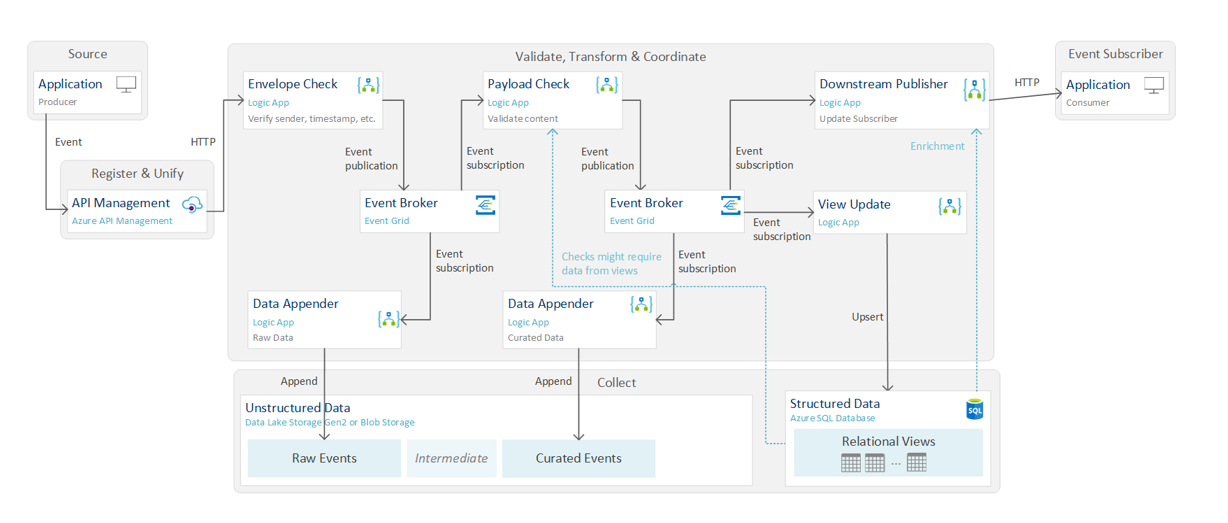
\includegraphics[width=\linewidth]{../img/Workflow.PNG}
\end{figure}

Eén van de belangrijkste punten van het Delaware Integration Platform, zoals dit framework genoemd wordt, is de mogelijkheid om verschillende applicaties te integreren en dan samen te gebruiken. Dit valt terug te vinden in bijlage B.2 DIP Het blootstellen van data vanuit het platform naar verschillende klanten met beveiligde API's is hierbij een vereiste. In dit geval zijn de klanten dan bedrijven, processen, mobiele apparaten of andere third-party gebruikerinterfaces. Met API enablement, kunnen API's gepubliseerd, gemanaged en beveilgd worden. De Data-Accelerator speelt dus ook vooral hier op in.

Om kort een beeld te schetsen van de Data-Accelerator kan men onderstaand bijlage B.3 Data-Accelerator bekijken. Hierin kan men zien dat er twee data producers zijn, deze sturen elkaar data door die dan bijgehouden wordt in een master data object. Deze raw data wordt dan omgezet naar modellen om van daar uit de benodigde data via de Data-Accelerator naar een Operation Data Store te brengen oftewel een kant en klare databank. Echter kan via de Data-Accelerator ook via Rest-API functies, ook data doorgegeven of opgehaald worden bij consumers, dit zijn dan andere functies die met de gespecifieerde data willen werken.

